\part{Rapport d'alternance}
\label{prt:missions} % utilisé pour faire des références dans le texte, pas besoin d'écrire le nom ou le numéro de la partie on donne juste le nom et lui il se charge de le remplacer par le nom

%\chapter{GROUPAMA GAN VIE (GGVie)}
GROUPAMA GAN VIE \footnote{ Description disponible sur http://www.groupama.com/fr/fiche/groupama-gan-vie/} (GGVie) est la société vie unique du groupe GROUPAMA. Elle assure la conception, la souscription et la gestion des contrats d'assurances de personnes (épargne, retraite, prévoyance et santé) commercialisés par les cinq réseaux de distribution du Groupe (les Caisses régionales, Gan Assurances, Gan Patrimoine, Gan Prévoyance et le courtage). Elle est organisée autour de deux directions métiers - Individuelle et Collective - et de trois directions fonctionnelles (Affaires générales et risque management, Financière, Ressources Humaines et Communication interne).

Mon alternance s'est déroulé au sein du service de veille réglementaire et technologique (SVRT). Sous la direction financière, le service veille essentiellement à l'application des différentes normes auxquelles est soumise la société donc Solvabilité \textsc{II}. Ses principales missions sont :
\begin{itemize}
\item S'assurer du respect des processus de calcul et des quantités réglementaires.
\item De la gestion actif-passif relative à l'ORSA (Own Risk and Solvency Assessment) de Solvabilité \textsc{II}
\item Des reportings réglementaires \textsc{II}.
\item De la recherche et de la promotion de nouveaux outils open source pour l'actuariat.
\end{itemize}

En tant que chargé d'études actuarielles au sein du service, j'étais en charge de la veille technologique. J'avais pour mission de trouver des nouveaux outils open source et méthodes fiables qui faciliteront le travail quotidien de l'actuaire, d'effectuer des test et aussi éventuellement des migrations de processus de calcul vers python, qui est un langage qui gagne de plus en plus en succès dans le monde de l'assurance et de la finance.

\chapter{Python et langage C : Cython} 

Ma première mission était de comprendre le fonctionnement d'un langage de programmation dérivé de python, le cython.

Python est un langage de programmation conçu en 1991 par Guido van Rossum, un développeur néerlandais. Aujourd'hui, c 'est la Python Software Foundation, une organisation à but non lucratif particulièrement dévouée, créée en 2001, qui est en charge de l'évolution du langage. Ce langage a été baptisé ainsi en hommage à la troupe de comiques les « Monty Python »\footnote{source : openclassroom}.

\section{Python}

Python est un langage libre cross-platform qui doit son succès à sa lisibilité, son multi-paradigme et ses multiples bibliothèques. Python défie désormais les célèbres logiciels R et SAS dans les domaines de la science de données et du machine learning, et aussi les logiciels de calcul numériques tels Matlab. Cependant python est un langage interprété, ce qui lui confère une bien moins bonne réputation en terme de rapidité d'exécution que les langages compilé tels que le C et le fortran. Pour combler cette faiblesse, une communauté de développeur on créé \emph{Cython}.

\section{Cython}

Le langage cython est une extension du langage python qui étend les possibilités de python, à la déclaration de variable et l'utilisation de fonctions C. 
Un projet cython contient au minimum trois fichiers avec différentes extensions:
\begin{itemize}
\item  \textbf{.pyx} : qui contient le code cython
\item  \textbf{setup.py} : qui contient les instructions de compilation du code cython.
\item \textbf{.py} :  qui importe et exécute le script cython compilé dans un fichier d'extension \textbf{.so} (linux) et \textbf{.pyd} windows.
\end{itemize}

Le code cython doit être compilé en deux étapes avant d'être exécutable : 
\begin{itemize}
\item le fichier \textbf{.pyx} est d'abord compilé et transformé en code C par l'extension cython installé sur python.
\item ensuite le fichier \textbf{.c} obtenu (à l'étape précédente) est compilé par un compilateur C en un fichier \textbf{.so} (linux) ou \textbf{.pyd} (windows), qui peut ensuite être importé dans un code python.
\end{itemize}

En résumé, python devient capable d'utiliser les outils et les propriétés du langage C. 

\section{Programmer en Cython}

\subsection{Installation de cython}

Pour utiliser le langage cython il faut installer le package pour python du même nom.

\begin{minted}[linenos=true]{python}
pip install cython
\end{minted}

\subsection{Exemple : helloword}

Prenons un exemple de programme cython qui affiche le message "Hello World" à l'écran. Il permettra de présenter les différentes étapes de mise en œuvre d'un projet cython.

\subsubsection{Code cython}
Dans le fichier hello.pyx qui contient le cython on aura:
\begin{minted}[linenos=true, fontsize=\footnotesize]{python}
print "Hello World"
\end{minted}


\subsubsection{Instructions de compilation}
Dans le fichier setup.py qui contient contient les instructions de compilation on aura :

\begin{minted}[linenos=true, fontsize=\footnotesize]{python}
from distutils.core import setup
from Cython.Build import cythonize

setup(
  name = 'Hello world app',
  ext_modules = cythonize("hello.pyx"),
)
\end{minted}

\subsubsection{Compilation}
Ensuite il faut compiler le code cython à l'aide d'un compilateur C. A partir d'un terminal on entre l'instruction suivante:

\begin{minted}[linenos=true, fontsize=\footnotesize]{python}
python setup.py build_ext --inplace
\end{minted}

La compilation génère un fichier \textbf{hello.so} si on est sous linux ou \textbf{hello.pyd} si on est sous windows. Le fichier généré peut ensuite être importé dans une session python.
Il faut noter qu'il existe plusieurs manières de compiler du code cython, ces différentes méthodes de compilation sont disponibles dans la documentation\footnote{http://cython.org/\#documentation} de cython.

\subsubsection{Exécution du code cython}
Pour exécuter le code cython, il faut importer le fichier \textbf{.so} ou \textbf{.pyd} dans une session ou code python.
\begin{minted}[linenos=true, fontsize=\footnotesize]{python}
>>> import hello
Hello World
\end{minted}

Le fonctionnement de cython sous entend qu'il traduit du code python en code C qui sera ensuite compilé. Cela sous entend aussi qu'il est capable de convertir les bibliothèques python. Mais toutes les bibliothèques ne sont pas encore prises en charge par python, c'est à dire que cython ne saura pas traduire le code python de certaine bibliothèque en code C.

%%%%%%%%%%%%%%%%%%%%%%%%%%%%%%%%%%%%%%%%%%%%%%%%%%% CHAP 2 %%%%%%%%%%%%%%%%%%%%%%%%%%%%%%%

\chapter{Reporting Solvabilité II et Datavizualisation}

Solvabilité II\footnote{http://acpr.banque-france.fr/solvabilite2.html} est une réforme européenne de la réglementation prudentielle s’appliquant au secteur de l'assurance, et en vigueur depuis le $1^{er}$ janvier 2016.
Elle vise à encourager les compagnies d'assurance à adopter une gestion efficientes de leur propre risque en adéquation avec les exigences règlementaires.
Ces exigences sont structurées en trois piliers : 
\begin{itemize}
\item \textbf{Pilier I} : les exigences quantitatives, notamment en matière de fonds propres et du calcul des provisions techniques.
\item \textbf{Pilier II} : les exigences en matière d’organisation et de gouvernance des organismes.
\item \textbf{Pilier III} : les exigences en matière de publication d'informations prudentielles. 
\end{itemize} 

 Le contrôle des compagnies s'effectue au niveau national par Autorité de contrôle prudentiel et de résolution (ACPR) et au niveau européen par 
 l'European Insurance and Occupational Pensions Authority (EIOPA)
 
\section{Pilier 3 : Reporting}

Le pilier 3 de solvabilité 2 vise à une standardisation de la publication des informations financières et hypothèses ayant été utilisées pour les calculs aux deux premiers piliers.

Le pilier 3 permet entre autres:

\begin{itemize}
\item une meilleure activité de contrôle de l'état de solvabilité des compagnies d'assurance par l'autorité de contrôle
\item une standardisation de la publication des informations afin de les rendre accessible au niveau mondiale
\item Une comparaison, au niveau Européen, des compagnies d'assurance entre elles
\end{itemize}

Pour ce faire, les autorités de contrôle publient des maquettes qui se présentent sous la forme de tables Excel à remplir, accompagnées des différentes directive à suivre pour mener l’exercice à bien.

\subsubsection*{QRT : Quantitative Reporting Templates}

Les QRT sont des maquettes de tableaux excel, que les organismes d'assurance doivent remplir et soumettre à l'EIOPA. Ils sont publiés avec une documentation comportant l'ensemble des informations et les définitions sur les quantités à renseigner ainsi que les formules de calcul.

\subsubsection*{ENS :  États nationaux spécifiques : }
%reporting sur le site de l'acpr
Les QRT au niveau européen sont complétés par des exigences nationales pour devenir les états nationaux spécifiques (ENS). Les ENS permettent une adaptation des règles au contexte économique du pays.

\section{Description générale du reporting} 
 
L'ensemble des maquettes à remplir et leur documentation sont publiées sur les sites des différents contrôleurs. Le reporting réglementaire Solvabilité II consiste donc pour un assureur à :

\begin{itemize}
\item récupérer des maquettes, documentations et directives sur le site de l'autorité qu'il rempli en s'assurant de bien respecter les indications.
\item transformer ces fichiers excel (remplis) en fichiers \textbf{xbrl} , qui est un format de fichier standard pour la publication d'informations financières et comptables.
\end{itemize}

Le format xbrl est un format de fichier du type xml conçu pour le report de données comptables et financières. Les fichiers xbrl sont générés à partir de fichiers excels, et peuvent être automatiquement contrôlés à l'aide des taxonomies. Les  taxonomies sont comme des cahiers de charges ou assertions dans lesquels sont inscrites l'ensemble des logiques que doivent respecter les quantités dans le fichier xbrl. Les taxonomies se présentent sous la forme d'une succession 

Les taxonomies sont appliquées sur les fichiers xbrl pour vérifier le respect des règles. Parmi les assertions il existe les assertions dites bloquantes qui si une seule n'est pas respectée entraîne le rejet systématique du fichier par l'autorité de contrôle. Il y'a au moins 8500 assertions rien que pour les ENS. Autant dire que la difficulté ne se trouve pas le fait d'entrer des formules dans des cellules excel, mais obtenir un taux d'erreur de 0/8500.

C'est dans l'objectif de concevoir un outil qui permettrait de faciliter la vérification des assertions qu'est né la mission de datavisualisation.

La mission consistait à écrire un programme python qui génère automatiquement à partir de la liste des assertions un fichier de type json avec un format bien particulier. le fichier de type .json ira à son tour alimenter un graphique web dynamique  généré à l'aide la bibliothèque javascript d3js.
Le graphique généré est un graphe qui permet de visualiser de façon intuitive les assertions.

\begin{figure}[H]
\centering
\caption{Graphes des liens entre les QRT}
   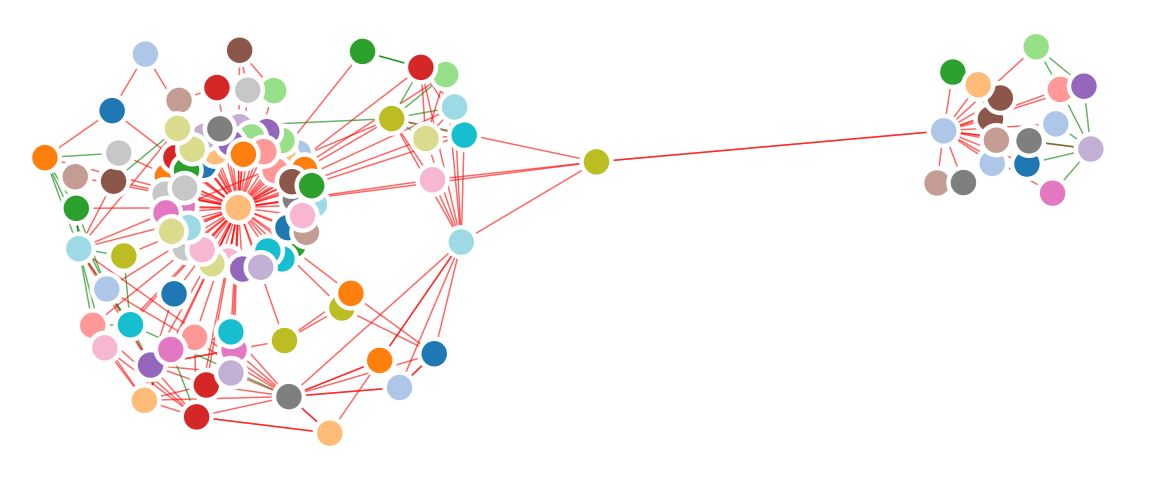
\includegraphics[scale=0.5]{img/graph.JPG}
\end{figure}

Quelques précision sur le graphe : 
\begin{itemize}
\item Le graphe est dynamique, et un pointage du curseur sur un  nœud affiche le nom du QRT représenté.
\item la distance entre deux noeuds matérialise la force de leur lien. Plus les noeuds sont proche, plus ils existent des assertions qui relient ces QRT.
\end{itemize}

Ce graphe permet une représentation visuelle de l'ensemble des liens qui existent entre les QRT. A l'aide de ce graphe il est possible de distinguer les QRT centraux, c'est à dire ceux qui auront tendance à être la base des autres, et de pouvoir bien définir un ordre cohérent de remplissage des QRT afin d'éviter les erreurs.




\chapter{De SAS à Python}

Le logiciel utilisé pour réaliser l'inventaire, est SAS. Cependant la licence du logiciel ne sera pas systématiquement renouvelée pour tous les collaborateurs et python a été choisi comme alternative. Ainsi un des grands prochains chantier du service sera la migration du code SAS existant vers python, et d'en faire le langage spécial inventaire.

Pour décrire un peu l'inventaire, il consiste à faire l'état du portefeuille client, et de calculer certaines variables techniques (provision mathématiques, provision zillmérisées...) pour chaque assuré. C'est donc un ensemble de requête SQL et de manipulations de données (ajout de colonnes, groupes, jointures).

Le but de la mission est de tester la faisabilité du chantier. Il s’agissait de comprendre l’ensemble des traitements effectués pour réaliser les inventaires avec SAS, s'assurer qu'ils sont réalisables sous python et de savoir comment les implémenter. 

Pour réaliser du traitement de données, il y a pandas. Pandas est une bibliothèque python pour la manipulation de données, c'est Wes McKinney, un statisticien américain qui en est le principale auteur. Ainsi toutes les manipulations qu'offre SAS pour l'inventaire sont réalisables sous python.

Une fois le code SAS qui fait l'inventaire compris, j'ai écrit quelques échantillons de traduction python documentés, ensuite j'ai effectué une petite formation python du collaborateur en charge de cette tâche de migration du code SAS vers python.

\chapter{Participation au bénéfice}

Le code\footnote{https://www.legifrance.gouv.fr/} des assurances à l'article L 331-3 stipule :
"Les entreprises d'assurance sur la vie ou de capitalisation doivent faire participer les assurés aux bénéfices techniques et financiers qu'elles réalisent, dans les conditions fixées par arrêté du ministre de l'économie et des finances."

Ainsi GGVie est en tant que société d'assurance vie, calcul chaque année la participation au bénéfice réglementaire qu'elle devra verser à ses assurés. 

\section{Calcul de la participation au bénéfice réglementaire ou PBR}

L'objectif de cette mission était de concevoir un programme python qui calcule la participation au bénéfice réglementaire en utilisant pour seul paramètre d'entrée la balance\footnote{La balance est un journal comptable dans lequel est répertorié l'ensemble des flux financiers liés à l'activité de la société d'assurance vie.}.

Le calcul de la participation au bénéfice réglementaire, se fait à partir d'un compte de participation au résultat qui se présente comme suit : 

\begin{table}[H]
\centering
\caption{Compte de participation aux résultats}
\label{CPR}
\begin{tabular}{|l|L{9cm}|L{4cm}|}
\hline
 & \multicolumn{1}{c|}{RUBRIQUE}  & \multicolumn{1}{c|}{COMMENTAIRES} \\ \hline
1 & Primes &  \\ \hline
2 & Charges des prestations &  \\ \hline
3 & Charge des provisions d'assurance Vie et des autres provisions techniques &  \\ \hline
A. & Solde de souscription (2) & 1-2-3 \\ \hline
5 & Frais d'acquisition &  \\ \hline
6 & Autres charges de gestion nettes & 5+6 \\ \hline
B & Charges d'acquisition et de gestion nettes &  \\ \hline
Gt & Participation de l'assureur aux bénéfices de la gestion techniques (A 331-4) & Gt = 10\% de (A-B) si A-B >0. Gt = 0 si A-B<0 \\ \hline
Pf & Part des produits financiers & Pf = 85\% du solde du compte financier \\ \hline
R & Solde de réassurance cédée &  \\ \hline
N & Solde débiteur du compte de participation aux résultats de l'exercice précédent &  \\ \hline
Sr & Solde du compte de participation aux résultats & A - B - Gt + Pf + R - N \\ \hline
lt & intérêts crédités aux provisions mathématiques &  \\ \hline
Mm & Montant minimal annuel de la partcipation aux bénéfices & Mm = Sr - It \\ \hline
\end{tabular}
\end{table}

Les rubriques du tableau \ref{CPR} \footnote{\cite{Befec-PriceWaterhouse1996}} peuvent être obtenues à partir du compte de résultat et leurs calculs sont définis par le code des assurances.
Le calcul de la participation au bénéfice fait intervenir à la fois l'actif notamment la rentabilité des actifs, et le passif notamment les intérêt techniques. La PBR se présente ainsi comme un lien direct entre l'actif et le passif dont il faut tenir compte dans la projection du bilan. La PBR est ainsi une des liaisons majeures dont il faut tenir compte dans la gestion actif passif.

\section{Calcul de la PBR avec python}

Le calcul de la PBR se fait dans un classeur excel alimenté par plusieurs classeurs à leurs tours alimentés par des équipes différentes. Cependant cette méthode présente la conséquence d'un procédé long, impliquant plusieurs intermédiaires résultant sur un  risque aggravé d'erreur de calculs. C'est un effet araignée avec risque d'erreur non négligeable.

L'objectif est donc d'écrire un programme python qui élimine l'ensemble de ces intermédiaires, qui se contente de la balance en entrée, pour calculer la PBR.

Pour commencer, j'ai élaboré le compte de résultat à partir de sa maquette\footnote{La maquette du compte de résultat est un tableau qui associe chaque poste du compte de résultat aux comptes qui la compose.}. 
Ensuite à partir du compte de résultat il reste à construire le compte de participation aux résultats.

Cependant, certaines rubriques du compte de participation aux résultats ne sont pas explicites dans le compte de résultat, il faut donc faire une correspondance entre les rubriques des deux comptes. Une tache pas très aisé du fait qu'il est difficile de trouver des personnes sources unanimes sur les poste ou comment les calculer.

Une autre approche consiste à décortiquer les classeurs excel déjà en place qui calculent la PBR. c'est long et fastidieux, et en plus dans certains classeurs les cellules sont en "durs" plutôt que calculées. Conséquence, on se retrouve avec des quantités que l'on ne sais pas calculer. Et lorsque l'on se réfère au compte de participation au résultat pour calculer ces quantités, on se retrouve avec le problème de vocabulaire.

%\ref{CPR} que dans les classeurs excel déjà présents qui calculent la PBR.

Par exemple le solde de souscription dans le tableau \ref{CPR} est calculé différemment du solde de souscription dans les classeurs. En outre, le solde de souscription est appelé intérêt technique dans certains classeurs.

En résumé, il n'existe pas un vocabulaire explicite, entre la maquette du compte de résultat, le code des assurances, et des différents classeurs déjà utilisés pour calculer.

De cette mission, que l'on peut se retrouver avec des missions qui paraissent simples au départ, mais qui finissent par se révéler très complexe au point de déboucher dans des impasses toutefois possible à contourner.

\chapter{Le Challenge R de Groupama}

La direction internationale du Groupe GROUPAMA a lancé au début de l'année 2017 un concours de data science entre toutes les entités et filiales du groupe, baptisé le "Challenge R". L'idée de ce concours était de permettre aux différentes entités de développer eux même une solution à un problème concret tout en utilisant des outils open source et des techniques de statistiques et d'apprentissage automatique.

Le service de veille réglementaire et technologique a représenté GGVie au Challenge R. Ayant été soumis à des problèmes de données anormaux dans les tâches de gestion actif-passif, mon tuteur a donc eu l'idée d'un outils de détection d'anomalies dans des données en utilisant des méthodes d'apprentissage automatique. J'étais donc chargé de la mise en oeuvre en python et de la recherche de toutes méthode ou technique pouvant mener à un modèles robuste et fiable.

\section{Modélisation du passif avec MoSes}

La modélisation du passif consiste à projeter le portefeuille d'une ou plusieurs polices d'assurance sur quarante (40) ans, dans le but d’observer l'évolution des postes du passif, et d'anticiper les engagements et les rendements futurs.
Une sortie de modélisation du passif d'une police d'assurance, sera un ensemble de séries chronologiques, chacune représentant la projection d'un poste du passif de cette police sur une quarantaine d'année. 
A titre d'exemple, considérons la police d'assurance AX1, la modélisation de son passif sur 40 ans aura la forme suivante :

% Ce tableau est utilisé pour donner un aperçu du type de données obtenu en sortie de modèle

\begin{table}[H]
\centering
\caption{Passif de la police d'assurance \textsc{AX1}}
\label{my-label1}
\begin{tabular}{|l|l|l|l|}
\hline
    &  2018   &  2019   &  20..  \\ \hline
 MARGE TECHNIQUE   &  .   &   .  &  ...  \\ \hline
 PROVISIONS TECHNIQUES  &  .   &  .   &  ...  \\ \hline
 CHARGE DE PARTICIPATION AUX BENEFICES  &   .  &   .  &  ...  \\ \hline
  ...  &  .   &  .   &   ... \\ \hline
\end{tabular}
\end{table}

La projection du passif se fait avec le logiciel de gestion actif-passif MoSes de chez Towers Watson. Afin de fournir des projections, MoSes prend comme données d'entrée :

\begin{itemize}
\item le portefeuille dont on désire projeter le passif dans le temps
\item un ensemble d'hypothèses qui se présente sous la forme de tableaux de probabilité qu'un assuré change d'état d'une année à l'autre.
\end{itemize}

Pour chaque année de projection, MoSes applique les hypothèses au portefeuille pour simuler les changements d'états (décès, invalidité, incapacité...) des assurés d'une année à l'autre. Pour chaque année de projection, une simulation des flux de trésorerie engendrés par les variations de  portefeuille permet de construire le passif correspondant. 

\section{Problématique}

La modélisation de l'ensemble des polices pour un même poste du passif présente parfois des sorties "étonnantes", on peut observer des particularités chez certaines séries pour un même poste de passif comme : 

\begin{itemize}
\item des séries chronologiques avec des sauts
\item des valeurs nulles en plein milieu de série
\item des séries aux tendances différentes 
\item ...
\end{itemize}

Ces erreurs dans les résultats de modélisation peuvent engendrer des écarts de prévision et de gestion des risques, d'où l'idée de construire un modèle de détection d'anomalie qui sera présenté au concours de data science.

Ce modèle, baptisé "Garbage in, Garbage out" (G.I.G.O.), s'inscrit dans un objectif de fiabilisation des données.

\section{Garbage in, Garbage out (GIGO)}

GIGO est un modèle qui détecte les anomalies dans les résultats de modélisation du passif en se basant sur la forme générale de toute les séries chronologiques.

La construction du modèle s'est effectuée essentiellement sous deux approches partant de différentes hypothèses et interprétation afin de construire un modèle fiable et performant. 

\subsection{Approche basé sur la forme générale des courbes chronologiques}

La première approche a consisté à supposer que la détection pourrait se faire à partir de la forme générale des courbes des séries chronologiques. 

Supposons un ensemble de simulation d'un poste du passif pour 50 produits d'assurance différents. On aura donc 50 séries chronologiques, chacune représentant la projection dans le temps de différents produits pour un même poste du passif.

Chaque série présentera donc une forme générale, elle seront soit croissantes, décroissantes, convexes, concaves, ou une combinaison de ces formes.

\subsubsection{Détection des formes : le modéle de Nielson-Siegel-Svensson}

Partant de l'objectif d'une détection de séries anormales basée sur leurs formes, la première étape consistera donc à modéliser la forme générale des courbes. Pour ce faire, on utilisera le modèle de Nielson-Siegle-Svensson (NSS).

Le modèle de Nielson-Siegel-Svensson (NSS) est une extension du modèle de Nelson and Siegel (1987) par Svensson (1994), il est utilisé par la Banque Centrale Européenne (BCE) pour construire la courbe des taux. 

Le modéle propose une modélisation de la courbe des taux en fonction des maturités par l'équation\footnote{\cite{ManfredGilli2010}} :

\begin{multline}
y(\tau)=\beta_{0}+\beta_{1}\left[\frac{1-exp(\frac{-\tau}{\alpha_{1}})}{\frac{\tau}{\alpha_{1}}}\right]+\beta_{2}\left[\frac{1-exp(\frac{-\tau}{\alpha_{1}})}{\frac{\tau}{\alpha_{1}}}-exp(\frac{-\tau}{\alpha_{1}})\right]+ \\
\beta_{4}\left[\frac{1-exp(\frac{-\tau}{\alpha_{2}})}{\frac{\tau}{\alpha_{2}}}-exp(\frac{-\tau}{\alpha_{2}})\right]
\label{nss}
\end{multline}

Ainsi la calibration du modèle se fait par l'estimation des paramètres : $ \beta_{0},\beta_{1},\beta_{2},\beta_{3},\alpha_{1},\alpha_{2}. $ (Avec $ \tau $ la maturité)

Le modèle est à la base destiné à résoudre un problème de finance. Cependant, il présente un aspect qui nous permet de l'adapter à notre contexte de détection d'anomalies. En effet les paramètres $ \beta_{0},\beta_{1},\beta_{2},\beta_{3},\alpha_{1},\alpha_{2}. $  représentent chacun un aspect de la forme de la courbe modélisée. Ainsi, nous pouvons supposer que ces six paramètres résument bien la forme générale de la courbe qu'elle modélise. 

Pour revenir à notre contexte, nous pouvons donc résumer une série chronologique d'une quarantaine de points à six paramètres essentiels qui traduisent sa forme.

\subsubsection{Adaptation au modèle NSS}

Le modèle NSS a été construit afin de modéliser la courbe des taux en fonction de leur maturité. Dans notre contexte nous avons des quantité de passifs de l'ordre de plusieurs millions. Ainsi pour se conformer au modèle, il est nécessaire de ramener ces quantités à une échelle de taux (entre -1 et 1), et de ramener les années à des maturités.

\subsubsection{Calibration du modèle NSS}

Afin de trouver les six paramètres il faut procéder par la calibration du modèle. La calibration du modèle se fait par optimisation, il faut trouver les paramètres qui font passer la courbe de la fonction \eqref{nss} au mieux par l'ensemble des points de la série chronologique. 

Pour estimer les six paramètres on résout le problème d'optimisation qui consiste à minimiser les distances entre la fonction de NSS et les points à interpoler. La fonction objective sera donc :

\begin{equation}
min\sum_{k=1}^n (y_{nss}-y_{obervation})^{2}
\label{obj}
\end{equation}

sous les contraintes : $ \beta_{1} > 0; \lambda_{1,2} > 0; \beta_{1}+\beta_{2}>0 $

Le problème d'optimisation n'est pas convexe, une méthode "classique" de résolution se limiterait à trouver des optimum locaux. C'est pourquoi une méta-heuristique\footnote{"Une métaheuristique est un algorithme d’optimisation visant à résoudre des problèmes d’optimisation difficile" : https://fr.wikipedia.org/wiki/Métaheuristique}, en l’occurrence l'évolution différentielle\footnote{Rainer STORN and Kenneth PRICE : "Differential Evolution – A Simple and Efficient Heuristic for Global Optimization over Continuous Spaces", 1997} sera utilisée afin de trouver un optimum global.

En appliquant la méthode d'évolution différentielle afin de minimiser la fonction objective, on obtient comme solution le vecteur des six paramètres.

Appliquer le modèle NSS aux séries chronologiques revient à les réduire à six principaux paramètres qui résument au mieux leur forme.
\subsubsection{Application de NSS}

Soit la série chronologique suivante...

\begin{figure}[H]
\centering
\caption{Série chronologique normalisée}
   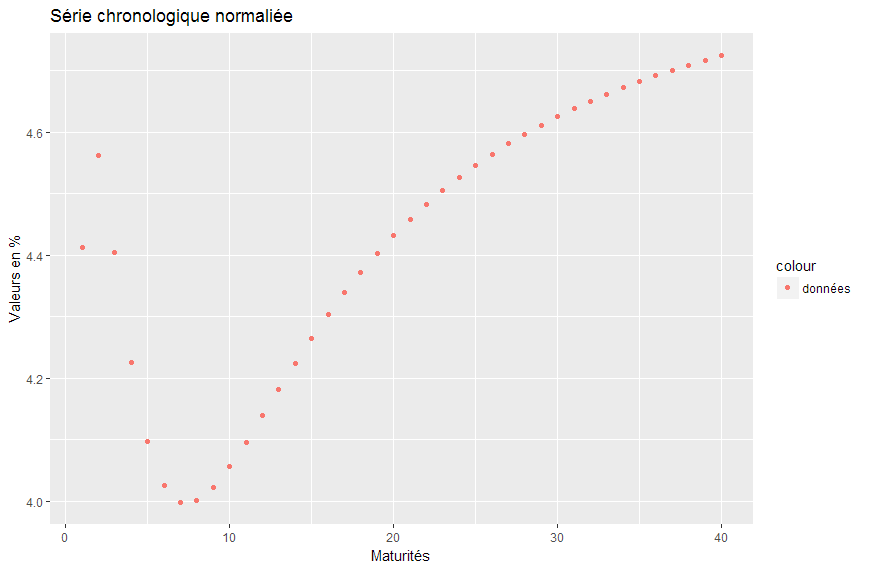
\includegraphics[scale=0.7]{img/data.png}
\end{figure}

En calibrant NSS sur ces données, on peut en déduire sa forme principale, à partir des six paramètres du modèle de nielson Siegel Svensson que l'on obtiendra.

Après calibration on obtient les six paramètres de l'équation de NSS, à partir de ces six paramètres et des maturités on recalcule les valeurs de la séries normalisée afin d'évaluer de façon graphique les performances de la calibration. En superposant les série normalisée initiale et la série obtenue par estimation de NSS, on obtient le graphique suivant :

\begin{figure}[H]
\centering
\caption{Série chronologique normalisée reprise par le modèle NSS}
   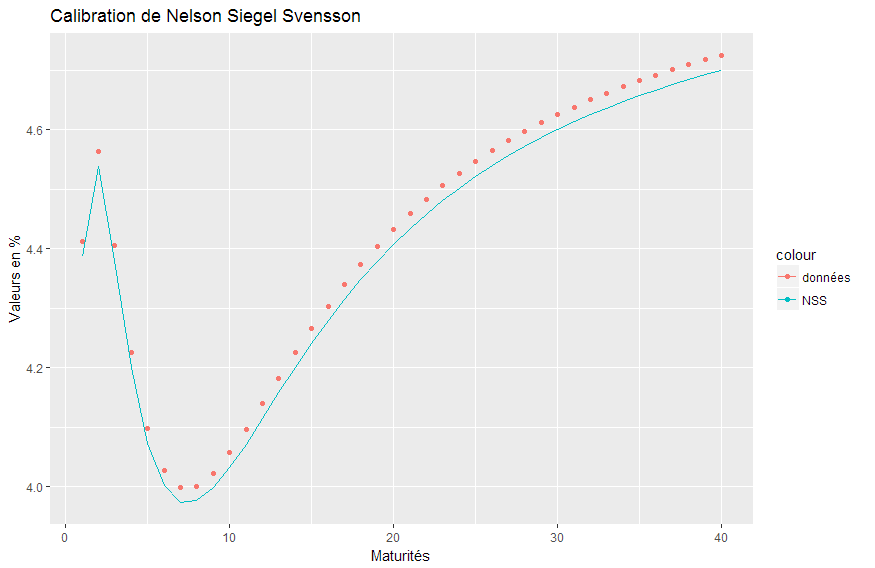
\includegraphics[scale=0.7]{img/nss.png}
\end{figure}

Les six paramètres optimaux de l'équation de NSS, obtenues à partir de la calibration du modèle sont : 

\begin{table}[H]
\centering
\caption{Paramètres optimaux}
\label{my-label}
\begin{tabular}{|l|r|l|l|l|l|l|}
\hline
$\beta$ & $\beta_0$ & $\beta_1 $ & $\beta_2$ & $\beta_3$ & $\alpha_1$ & $\alpha_2$ \\ \hline
Valeurs & 5 & -2 & 5 & -5 & 1 & 3 \\ \hline
\end{tabular}
\end{table}

Sans passer par tous les points, le modèle trace une qui courbe épouse bien la l'allure de la forme de la série chronologique normalisée, comme une ombre. Ainsi on déduit que le modèle de NSS viens de réduire à six paramètres la forme d'une courbe de quarante points.

Maintenant évaluons notre déduction en testant l'effet de changement de chacun des paramètres sur la courbe obtenue tracée par les paramètres. L'idée est de confirmé, qu'un changement de paramètre abouti à une nouvelle courbe d'un forme plus ou moins différente.

En effectuant successivement un changement de l'un des six paramètres afin d'évaluer le changement de courbe obtenu, on obtient les graphiques suivants :

\begin{figure}[H]
\centering
\caption{Conséquences des changements de paramètres}
   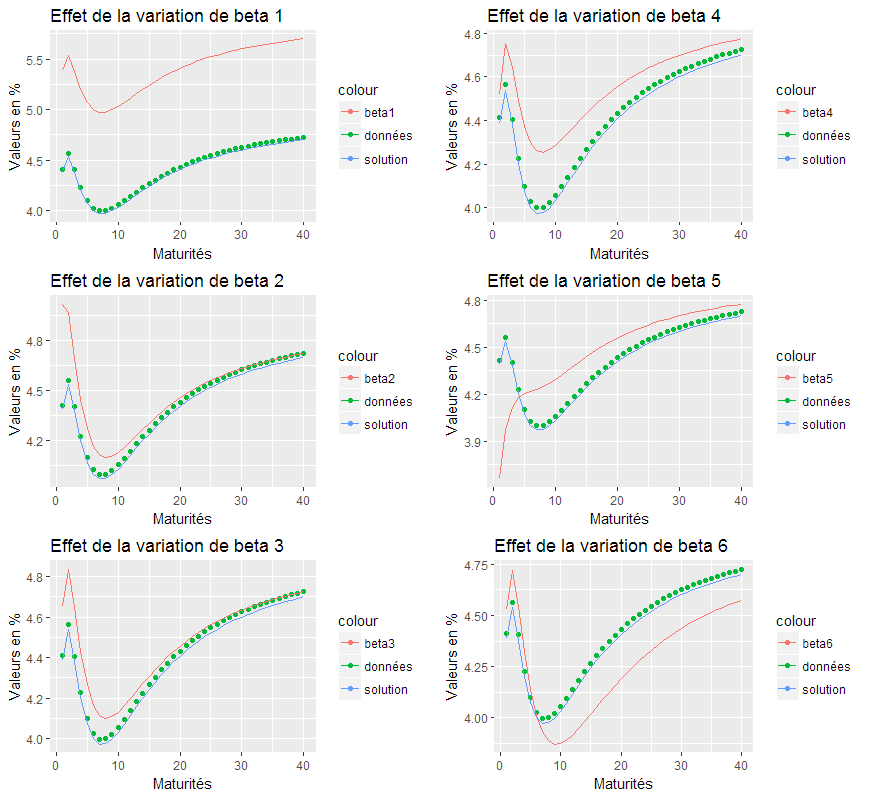
\includegraphics[scale=0.7]{img/betas.png}
\end{figure}

La modification qui a été faite est que l'on a successivement ajouté à chaque paramètre la valeur de 1.
Pour chaque paramètre modifié, on observe bien certains changements dans la forme de la courbe, ce qui signifie bien que les six paramètres permettent de caractériser une courbe particulière.

En résumant une courbe à ses six paramètres, on effectue une réduction de dimension, mais aussi un changement de repère, on passe des valeurs de la courbe, à la forme de la courbe. Ainsi, calculer la distance entre les paramètres de deux courbes différentes reviendrait à calculer la différence qui existe entre les formes de leurs courbes respectives.

\subsubsection{Détection}

Après avoir identifié la forme de la courbe de chaque série, on passe maintenant à la phase de détection d'anomalies. La détection d'anomalie est un procédé utilisé dans des domaines divers, dans le but essentiel d'isoler des comportements ou des individus "suspects" dans un ensemble de données ou d'activités.

Il existe une multitude de méthode de détection d'anomalies, toutes  généralement basées sur les calculs de distances et de noyaux. La méthode que nous allons utiliser procède à la détection par isolation.

\subsection{Approche basée sur les séries chronologiques}

Par cette approche on procède directement à l'application de la méthode de forêt d'isolation pour détecter les anomalies, sans étape intermédiaire en supposant que les années de projection sont des variables. Cette approche sera développée dans la seconde partie.

L'objectif de la seconde partie sera de présenter l'aspect théorique et pratique, montrant les performances et l'intérêt de cette méthode de détection utilisée dans un contexte de la finance de marché.


%In this section, we will deal with the optimisation problem, so our aim will be to solve
%model (3). The problem is not convex, so we will use appropriate procedures: optimisation
%heuristics (Gilli and Winker, 2009). More specifically, we will apply Differential Evolution
%(de; Storn and Price, 1997). We will not discuss the algorithm in detail here; the implementation
%follows the pseudocode given in Gilli and Schumann (2010 (in press). R-code is given
%in the appendix and can be downloaded from http://comisef.eu .
% part  (end)/